\documentclass{beamer}
\usepackage[utf8]{inputenc}
\usepackage[english]{babel}
\usepackage[T1]{fontenc}
\usepackage[inline]{asymptote}
\usepackage{pgfplots}
\pgfplotsset{compat=1.5} 
\usepgfplotslibrary{statistics}
\usepackage{tikz}
\usetikzlibrary{shapes,arrows}
\usepackage{slide_helper}

\title[MA205 - Section 3.3]{Measures of Relative Standing and Boxplots}

%% Define block styles
%\tikzstyle{decision} = [diamond, draw, fill=yellow!20, 
%    text width=4.5em, text badly centered, node distance=3cm, inner sep=0pt]
%\tikzstyle{block} = [rectangle, draw, fill=blue!20, 
%    text width=5em, text centered, rounded corners, minimum height=4em]
%\tikzstyle{line} = [draw, -latex']
%\tikzstyle{cloud} = [draw, ellipse,fill=red!20, node distance=3cm,
%    minimum height=2em]
%    
%\begin{tikzpicture}[node distance = 2cm, auto]
%    % Place nodes
%    \node [block] (init) {initialize model};
%    \node [cloud, left of=init] (expert) {expert};
%    \node [cloud, right of=init] (system) {system};
%    \node [block, below of=init] (identify) {identify candidate models};
%    \node [block, below of=identify] (evaluate) {evaluate candidate models};
%    \node [block, left of=evaluate, node distance=3cm] (update) {update model};
%    \node [decision, below of=evaluate] (decide) {is best candidate better?};
%    \node [block, below of=decide, node distance=3cm] (stop) {stop};
%    % Draw edges
%    \path [line] (init) -- (identify);
%    \path [line] (identify) -- (evaluate);
%    \path [line] (evaluate) -- (decide);
%    \path [line] (decide) -| node [near start] {yes} (update);
%    \path [line] (update) |- (identify);
%    \path [line] (decide) -- node {no}(stop);
%    \path [line,dashed] (expert) -- (init);
%    \path [line,dashed] (system) -- (init);
%    \path [line,dashed] (system) |- (evaluate);
%\end{tikzpicture}
    
\begin{document}
\begin{frame}
\titlepage
\end{frame}

\begin{frame}
\begin{definition}
A \textbf{$z$-score} is the number of standard deviations that a given value is above or below the mean.
\end{definition}\pause

\begin{block}{Formula}
The $z$-score for a given value $x$ is calculated as follows.
\begin{description}
\item[\textbf{Sample:}] $z=\dfrac{x-\bar{x}}{s}$
\item[\textbf{Population:}] $z=\dfrac{x-\mu}{\sigma}$
\end{description}
\end{block}\pause

\begin{block}{Properties}
\begin{itemize}[<+- | alert@+>]
\item $z$-scores are expressed as numbers with no units.
\item A data value is \emph{significantly low} if $z\leq -2$.
\item A data value is \emph{significantly high} if $z\geq 2$.
\item If a data value is less than the mean, its $z$-score will be negative.
\end{itemize}
\end{block}
\end{frame}

\begin{frame}
\begin{example}
The weights of a sample of 400 newborn baby weights has mean $\bar{x}=\textcolor<3-4>{blue}{3152.0}$ g and standard deviation $s=\textcolor<3-4>{red}{693.4}$ g. What is the $z$-score of a \textcolor<3-4>{cyan}{4000} g baby?\pause

\vspace{-3mm}
\begin{equation*}
z=\dfrac{x-\bar{x}}{s}\pause
=\dfrac{\textcolor<3-4>{cyan}{4000}-\textcolor<3-4>{blue}{3152.0}}{\textcolor<3-4>{red}{693.4}}\pause
=1.22
\end{equation*}
\end{example}\pause

\begin{example}
The weights of a sample of 106 adult temperature has mean $\bar{x}=\degree{\textcolor<7-8>{blue}{98.20}}$F and standard deviation $s=\degree{\textcolor<7-8>{red}{0.62}}$F. What is the $z$-score of an adult with temperature $\degree{\textcolor<7-8>{cyan}{96.5}}$F?\pause

\vspace{-3mm}
\begin{equation*}
z=\dfrac{x-\bar{x}}{s}\pause
=\dfrac{\textcolor<7-8>{cyan}{96.5}-\textcolor<7-8>{blue}{98.20}}{\textcolor<7-8>{red}{0.62}}\pause
=-2.74
\end{equation*}
\end{example}\pause

\begin{block}{Rounding}
Round $z$-scores to two decimal places.
\end{block}
\end{frame}

\begin{frame}
\begin{definition}
\textbf{Percentiles} are measures of location, denoted $P_{1},P_{2},\ldots,P_{99}$, which divide a set of data into 100 groups with about $1\%$ of the values in each group.
\end{definition}\pause

\begin{block}{Formula}
The process of finding the percentile that corresponds to a particular data value $x$ is given by the following:
\begin{equation*}
\text{Percentile of value $x$} = \dfrac{\text{number of values less than $x$}}{\text{total number of values}}\cdot 100
\end{equation*}
\end{block}\pause

\begin{block}{Rounding}
Round percentiles to the nearest whole number.
\end{block}
\end{frame}

\begin{frame}
\begin{example}
The table lists the 50 Verizon airport data speeds, in Mbps, from\\ Data Set 32 in Appendix B.
\begin{center}
\begin{tabular}{rrrrrrrrrr}
38.5 & 55.6 & 22.4 & 14.1 & 23.1 & 24.5 & \textcolor<2->{blue}{6.5} & 21.5 & 25.7 & 14.7 \\
77.8 & 71.3 & 43.0 & 20.2 & 15.5 & 13.7 & \textcolor<2->{blue}{11.1} & 13.5 & \textcolor<2->{blue}{10.2} & 21.1 \\
15.1 & 14.2 & \textcolor<2->{blue}{4.5} & \textcolor<2->{blue}{7.9} & \textcolor<2->{blue}{9.9} & \textcolor<2->{blue}{10.3} & \textcolor<2->{blue}{6.2} & 17.5 & 22.2 & 13.1 \\
18.2 & 28.5 & 15.8 & 15.0 & \textcolor<2->{blue}{11.1} & \textcolor<2->{red}{11.8} & 16.0 & \textcolor<2->{blue}{10.9} & \textcolor<2->{blue}{1.8} & 34.6 \\
\textcolor<2->{blue}{4.6} & 12.0 & \textcolor<2->{blue}{11.6} & \textcolor<2->{blue}{3.6} & \textcolor<2->{blue}{1.9} & \textcolor<2->{blue}{7.7} & \textcolor<2->{blue}{0.8} & \textcolor<2->{blue}{4.5} & \textcolor<2->{blue}{1.4} & \textcolor<2->{blue}{3.2} \\
\end{tabular}
\end{center}
What percentile is the data value 11.8 Mbps in?\pause

There are 20 \textcolor{blue}{data values less than} \textcolor{red}{11.8} Mbps.\pause 

\vspace{-3mm}
\begin{equation*}
\text{Percentile of}~\textcolor{red}{11.8}=\dfrac{20}{50}\cdot 100\pause = 40
\end{equation*}

\vspace{-5mm}
A data speed of 11.8 Mbps is in the 40th percentile.
\end{example}\pause

\begin{block}{Note}
This can be interpreted loosely as 40\% of Verizon data speeds are slower than 11.8 Mbps and 60\% of Verizon data speeds are faster than 11.8 Mbps.
\end{block}
\end{frame}

\begin{frame}
\begin{block}{Converting a Percentile to a Data Value}
Notation:
\begin{itemize}
\item $n$ is the total number of values in the data set.
\item $k$ is the percentile being used.
\item $L$ is the locator that gives the position of a value.
\item $P_k$ is the $k$th percentile.
\end{itemize}\pause
To find which data value is in the $P_k$ percentile:
\begin{enumerate}
\item Sort the data from lowest to highest.\pause
\item Compute $L=\left(\dfrac{k}{100}\right)n$\pause
\item \begin{itemize}
\item If $L$ is a whole number, the value of the $k$th percentile is midway between the $L$th value and the next value in the sorted data. Add the $L$th value and $(L+1)$th value, then divide by 2.\pause
\item If $L$ is not a whole number, round $L$ up to the nearest whole number. $P_k$is the $L$th data value. 
\end{itemize}
\end{enumerate}
\end{block}
\end{frame}

\begin{frame}
\begin{example}
The table lists the \textcolor<4-5>{red}{50} Verizon airport data speeds, in Mbps, from\\ Data Set 32 in Appendix B.
\temporal<2-6>{%
\begin{center}
\begin{tabular}{|rrrrrrrrrr|}\hline
38.5 & 55.6 & 22.4 & 14.1 & 23.1 & 24.5 & 6.5 & 21.5 & 25.7 & 14.7 \\
77.8 & 71.3 & 43.0 & 20.2 & 15.5 & 13.7 & 11.1 & 13.5 & 10.2 & 21.1 \\
15.1 & 14.2 & 4.5 & 7.9 & 9.9 & 10.3 & 6.2 & 17.5 & 22.2 & 13.1 \\
18.2 & 28.5 & 15.8 & 15.0 & 11.1 & 11.8 & 16.0 & 10.9 & 1.8 & 34.6 \\
4.6 & 12.0 & 11.6 & 3.6 & 1.9 & 7.7 & 0.8 & 4.5 & 1.4 & 3.2 \\\hline
\end{tabular}
\end{center}
}{%
\begin{center}
\begin{tabular}{|rrrrrrrrrr|}\hline
0.8 & 1.4 & 1.8 & 1.9 & 3.2 & 3.6 & 4.5 & 4.5 & 4.6 & 6.2 \\
6.5 & 7.7 & 7.9 & 9.9 & 10.2 & 10.3 & 10.9 & 11.1 & 11.1 & 11.6 \\
11.8 & 12.0 & 13.1 & 13.5 & 13.7 & 14.1 & 14.2 & 14.7 & 15.0 & 15.1 \\
15.5 & 15.8 & 16.0 & 17.5 & 18.2 & 20.2 & 21.1 & 21.5 & 22.2 & 22.4 \\
23.1 & 24.5 & 25.7 & 28.5 & 34.6 & 38.5 & 43.0 & 55.6 & 71.3 & 77.8 \\\hline
\end{tabular}
\end{center}
}{%
\begin{center}
\begin{tabular}{|rrrrrrrrrr|}\hline
\textcolor<2->{blue}{0.8} &
\textcolor<2->{blue}{1.4} &
\textcolor<2->{blue}{1.8} &
\textcolor<2->{blue}{1.9} &
\textcolor<2->{blue}{3.2} &
\textcolor<2->{blue}{3.6} &
\textcolor<2->{blue}{4.5} &
\textcolor<2->{blue}{4.5} &
\textcolor<2->{blue}{4.6} &
\textcolor<2->{blue}{6.2} \\
\textcolor<2->{blue}{6.5} &
\textcolor<2->{blue}{7.7} &
\textcolor<2->{red}{7.9} &
\textcolor<2->{cyan}{9.9} &
\textcolor<2->{cyan}{10.2} &
\textcolor<2->{cyan}{10.3} &
\textcolor<2->{cyan}{10.9} &
\textcolor<2->{cyan}{11.1} &
\textcolor<2->{cyan}{11.1} &
\textcolor<2->{cyan}{11.6} \\
\textcolor<2->{cyan}{11.8} &
\textcolor<2->{cyan}{12.0} &
\textcolor<2->{cyan}{13.1} &
\textcolor<2->{cyan}{13.5} &
\textcolor<2->{cyan}{13.7} &
\textcolor<2->{cyan}{14.1} &
\textcolor<2->{cyan}{14.2} &
\textcolor<2->{cyan}{14.7} &
\textcolor<2->{cyan}{15.0} &
\textcolor<2->{cyan}{15.1} \\
\textcolor<2->{cyan}{15.5} &
\textcolor<2->{cyan}{15.8} &
\textcolor<2->{cyan}{16.0} &
\textcolor<2->{cyan}{17.5} &
\textcolor<2->{cyan}{18.2} &
\textcolor<2->{cyan}{20.2} &
\textcolor<2->{cyan}{21.1} &
\textcolor<2->{cyan}{21.5} &
\textcolor<2->{cyan}{22.2} &
\textcolor<2->{cyan}{22.4} \\
\textcolor<2->{cyan}{23.1} &
\textcolor<2->{cyan}{24.5} &
\textcolor<2->{cyan}{25.7} &
\textcolor<2->{cyan}{28.5} &
\textcolor<2->{cyan}{34.6} &
\textcolor<2->{cyan}{38.5} &
\textcolor<2->{cyan}{43.0} &
\textcolor<2->{cyan}{55.6} &
\textcolor<2->{cyan}{71.3} &
\textcolor<2->{cyan}{77.8} \\\hline
\end{tabular}
\end{center}
}
What is the value in the \textcolor<4-5>{blue}{25}th percentile, $P_{25}$?\pause

First, sort the data.\pause

We next need to compute
\begin{equation*}
L=\dfrac{k}{100}\cdot n\pause
=\dfrac{\textcolor<4-5>{blue}{25}}{100}\cdot \textcolor<4-5>{red}{50}\pause
=12.5\pause
\end{equation*}
Since $L=12.5$ is not a whole number, we round up to $13$.\pause

So, $P_{25}$ is the 13th data value, \textcolor<7->{red}{7.9} Mbps.
\end{example}
\end{frame}

\begin{frame}
\begin{definition}
\textbf{Quartiles} are measures of location, denoted $Q_1$, $Q_2$, and $Q_3$, which divide a set of data into four groups with about 25\% of the values in each group.
\end{definition}\pause

\begin{block}{Quartile Descriptions}
\begin{description}
\item[\textbf{First Quartile, $\boldsymbol{Q_1}$:}] Same value as $P_{25}$. It separates the bottom 25\% of the sorted values from the top 75\%.\pause
\item[\textbf{Second Quartile, $\boldsymbol{Q_2}$:}] Same as the $P_{50}$ and the median. It separates the bottom 50\% of the sorted values from the top 50\%\pause
\item[\textbf{Third Quartile, $\boldsymbol{Q_3}$}:] Same as $P_{75}$. It separates the bottom 75\% of the sorted values from the top 25\%.
\end{description}
\end{block}\pause

\begin{block}{Note}
Use the same procedure for calculating percentiles to calculate quartiles.
\end{block}
\end{frame}

\begin{frame}
\begin{definition}
The \textbf{interquartile range} (\textbf{IQR}) is $Q_3-Q_1$.
\end{definition}\pause

\begin{block}{Outliers}
A data value is often considered an outlier if
\begin{itemize}
\item  the data value is greater than $Q_3 + 1.5\cdot\textbf{IQR}$.
\item  the data value is less than $Q_1 - 1.5\cdot\textbf{IQR}$.
\end{itemize}
\end{block}\pause

\begin{definition}
The \textbf{semi-interquartile range} is $\tfrac{Q_3-Q_1}{2}$.
\end{definition}\pause

\begin{definition}
The \textbf{midquartile} is $\tfrac{Q_3+Q_1}{2}$.
\end{definition}\pause

\begin{definition}
The \textbf{10-90 percentile range} is $P_{90}-P_{10}$.
\end{definition}
\end{frame}

\begin{frame}
\begin{definition}
For a set of data, the \textbf{5-number summary} consists of the five values:
\begin{enumerate}
\item Minimum
\item $Q_1$
\item Median ($Q_2$)
\item $Q_3$
\item Maximum
\end{enumerate}
\end{definition}
\end{frame}

\begin{frame}
\begin{example}
The table lists, in order from lowest to highest, the 50 Verizon airport data speeds, in Mbps, from\\ Data Set 32 in Appendix B.

\vspace{-3mm}
\temporal<2-4>{%
\begin{center}
\begin{tabular}{|rrrrrrrrrr|}\hline
\textcolor{red}{0.8} & 1.4 & 1.8 & 1.9 & 3.2 & 3.6 & 4.5 & 4.5 & 4.6 & 6.2 \\
6.5 & 7.7 & 7.9 & 9.9 & 10.2 & 10.3 & 10.9 & 11.1 & 11.1 & 11.6 \\
11.8 & 12.0 & 13.1 & 13.5 & 13.7 & 14.1 & 14.2 & 14.7 & 15.0 & 15.1 \\
15.5 & 15.8 & 16.0 & 17.5 & 18.2 & 20.2 & 21.1 & 21.5 & 22.2 & 22.4 \\
23.1 & 24.5 & 25.7 & 28.5 & 34.6 & 38.5 & 43.0 & 55.6 & 71.3 & 77.8 \\\hline
\end{tabular}
\end{center}
}{%
\begin{center}
\begin{tabular}{|rrrrrrrrrr|}\hline
\textcolor{blue}{0.8} &
\textcolor{blue}{1.4} &
\textcolor{blue}{1.8} &
\textcolor{blue}{1.9} &
\textcolor{blue}{3.2} &
\textcolor{blue}{3.6} &
\textcolor{blue}{4.5} &
\textcolor{blue}{4.5} &
\textcolor{blue}{4.6} &
\textcolor{blue}{6.2} \\
\textcolor{blue}{6.5} &
\textcolor{blue}{7.7} &
\temporal<2>{\textcolor{blue}{7.9}}{\textcolor{red}{7.9}}{\textcolor{blue}{7.9}} &
\temporal<3>{\textcolor{cyan}{9.9}}{\textcolor{blue}{9.9}}{\textcolor{blue}{9.9}} &
\temporal<3>{\textcolor{cyan}{10.2}}{\textcolor{blue}{10.2}}{\textcolor{blue}{10.2}} &
\temporal<3>{\textcolor{cyan}{10.3}}{\textcolor{blue}{10.3}}{\textcolor{blue}{10.3}} &
\temporal<3>{\textcolor{cyan}{10.9}}{\textcolor{blue}{10.9}}{\textcolor{blue}{10.9}} &
\temporal<3>{\textcolor{cyan}{11.1}}{\textcolor{blue}{11.1}}{\textcolor{blue}{11.1}} &
\temporal<3>{\textcolor{cyan}{11.1}}{\textcolor{blue}{11.1}}{\textcolor{blue}{11.1}} &
\temporal<3>{\textcolor{cyan}{11.6}}{\textcolor{blue}{11.6}}{\textcolor{blue}{11.6}} \\
\temporal<3>{\textcolor{cyan}{11.8}}{\textcolor{blue}{11.8}}{\textcolor{blue}{11.8}} &
\temporal<3>{\textcolor{cyan}{12.0}}{\textcolor{blue}{12.0}}{\textcolor{blue}{12.0}} &
\temporal<3>{\textcolor{cyan}{13.1}}{\textcolor{blue}{13.1}}{\textcolor{blue}{13.1}} &
\temporal<3>{\textcolor{cyan}{13.5}}{\textcolor{blue}{13.5}}{\textcolor{blue}{13.5}} &
\temporal<3>{\textcolor{cyan}{13.7}}{\textcolor{red}{13.7}}{\textcolor{blue}{13.7}} &
\temporal<3>{\textcolor{cyan}{14.1}}{\textcolor{red}{14.1}}{\textcolor{blue}{14.1}} &
\temporal<4>{\textcolor{cyan}{14.2}}{\textcolor{blue}{14.2}}{\textcolor{blue}{14.2}} &
\temporal<4>{\textcolor{cyan}{14.7}}{\textcolor{blue}{14.7}}{\textcolor{blue}{14.7}} &
\temporal<4>{\textcolor{cyan}{15.0}}{\textcolor{blue}{15.0}}{\textcolor{blue}{15.0}} &
\temporal<4>{\textcolor{cyan}{15.1}}{\textcolor{blue}{15.1}}{\textcolor{blue}{15.1}} \\
\temporal<4>{\textcolor{cyan}{15.5}}{\textcolor{blue}{15.5}}{\textcolor{blue}{15.5}} &
\temporal<4>{\textcolor{cyan}{15.8}}{\textcolor{blue}{15.8}}{\textcolor{blue}{15.8}} &
\temporal<4>{\textcolor{cyan}{16.0}}{\textcolor{blue}{16.0}}{\textcolor{blue}{16.0}} &
\temporal<4>{\textcolor{cyan}{17.5}}{\textcolor{blue}{17.5}}{\textcolor{blue}{17.5}} &
\temporal<4>{\textcolor{cyan}{18.2}}{\textcolor{blue}{18.2}}{\textcolor{blue}{18.2}} &
\temporal<4>{\textcolor{cyan}{20.2}}{\textcolor{blue}{20.2}}{\textcolor{blue}{20.2}} &
\temporal<4>{\textcolor{cyan}{21.1}}{\textcolor{blue}{21.1}}{\textcolor{blue}{21.1}} &
\temporal<4>{\textcolor{cyan}{21.5}}{\textcolor{red}{21.5}}{\textcolor{blue}{21.5}} &
\textcolor{cyan}{22.2} &
\textcolor{cyan}{22.4} \\
\textcolor{cyan}{23.1} &
\textcolor{cyan}{24.5} &
\textcolor{cyan}{25.7} &
\textcolor{cyan}{28.5} &
\textcolor{cyan}{34.6} &
\textcolor{cyan}{38.5} &
\textcolor{cyan}{43.0} &
\textcolor{cyan}{55.6} &
\textcolor{cyan}{71.3} &
\textcolor{cyan}{77.8} \\\hline
\end{tabular}
\end{center}
}{%
\begin{center}
\begin{tabular}{|rrrrrrrrrr|}\hline
0.8 & 1.4 & 1.8 & 1.9 & 3.2 & 3.6 & 4.5 & 4.5 & 4.6 & 6.2 \\
6.5 & 7.7 & 7.9 & 9.9 & 10.2 & 10.3 & 10.9 & 11.1 & 11.1 & 11.6 \\
11.8 & 12.0 & 13.1 & 13.5 & 13.7 & 14.1 & 14.2 & 14.7 & 15.0 & 15.1 \\
15.5 & 15.8 & 16.0 & 17.5 & 18.2 & 20.2 & 21.1 & 21.5 & 22.2 & 22.4 \\
23.1 & 24.5 & 25.7 & 28.5 & 34.6 & 38.5 & 43.0 & 55.6 & 71.3 & \textcolor<5>{red}{77.8} \\\hline
\end{tabular}
\end{center}
}

\vspace{-3mm}
We can compute the following:

\vspace{-2mm}
\begin{equation*}
\begin{aligned}
\text{minimum} &= \textcolor<1>{red}{0.8}\pause \\
Q_1 &= \textcolor<2>{red}{7.9}\pause \\
Q_2 &= \textcolor<3>{red}{13.9}\pause \\
Q_3 &= \textcolor<4>{red}{21.5}\pause \\
\text{maximum} &= \textcolor<5>{red}{77.8}\pause
\end{aligned}
\end{equation*}
And so, the 5-number summary is $0.8~7.9~13.9~21.5~77.8$
\end{example}
\end{frame}

\begin{frame}
\begin{definition}
A \textbf{boxplot} is a graph of a data set that consists of a line extending from the minimum value to the maximum value, and a box with lines drawn at the first quartile $Q_1$, the median, and the third quartile $Q_3$.

\begin{center}
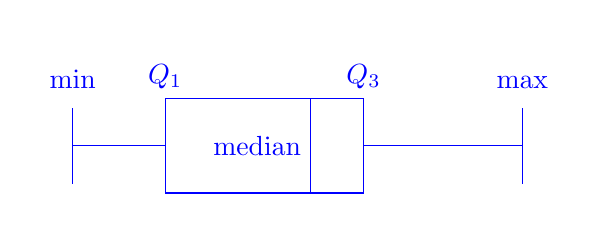
\begin{tikzpicture}
\begin{axis}[
y=1.5cm, 
ymax=2,
ytick=\empty,
xtick=\empty,
axis lines=none
]
\addplot+[
boxplot,
]
table[row sep=\\,y index=0] {
data\\
-2\\ 1\\ 2\\ 1\\ 5\\ 4\\ 10\\
7\\ 10\\ 9\\ 8\\ 9\\ 9\\ 15\\
}
[above]
node at
(boxplot box cs: \boxplotvalue{lower whisker},1)
{min}
node at
(boxplot box cs: \boxplotvalue{lower quartile},1)
{$Q_1$}
node[left] at
(boxplot box cs: \boxplotvalue{median},0.5)
{median}
node at
(boxplot box cs: \boxplotvalue{upper quartile},1)
{$Q_3$}
node at
(boxplot box cs: \boxplotvalue{upper whisker},1)
{max}
;
\end{axis}
\end{tikzpicture}
\end{center}
\end{definition}
\end{frame}

\begin{frame}
\begin{example}
The 5-number summary of the the 50 Verizon airport data speeds, in Mbps, from\\ Data Set 32 in Appendix B is:
\begin{equation*}
0.8\quad 7.9\quad 13.9\quad 21.5\quad 77.8
\end{equation*}

The boxplot is:
\begin{center}
\begin{tikzpicture}
\begin{axis}[
width=\linewidth,
height=5cm,
xlabel={},
ylabel={},
yticklabels={},
axis y line=none,
axis x line=bottom,
y=2cm,
xmin=0,
xmax=80,
]
\addplot+ [
boxplot prepared={
lower whisker=0.8,
lower quartile=7.9,
median=13.9,
upper quartile=21.5,
upper whisker=77.8,
},
]
table [row sep=\\,y index=0] {
data\\
};
\end{axis}
\end{tikzpicture}
\end{center}
\end{example}\pause

\begin{block}{Note}
A boxplot can often be used to identify skewness.
\end{block}
\end{frame}

\begin{frame}
\begin{example}
We can use boxplots to easily compare the four carriers from Data Set 32 in Appendix B.
\begin{center}
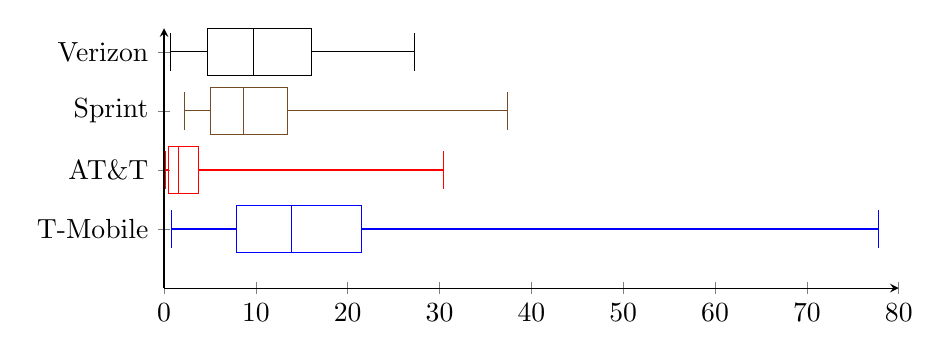
\begin{tikzpicture}
\begin{axis}[
width=0.9\linewidth,
%height=5cm,
xlabel={},
ylabel={},
axis y line=left,
axis x line=bottom,
y=0.75cm,
xmin=0,
xmax=80,
ymin=0,
ytick={1,2,3,4},
yticklabels={T-Mobile, AT\&T, Sprint, Verizon},
]
\addplot+ [
boxplot prepared={
lower whisker=0.8,
lower quartile=7.9,
median=13.9,
upper quartile=21.5,
upper whisker=77.8,
},
]
coordinates {};

\addplot+ [
boxplot prepared={
lower whisker=0.2,
lower quartile=0.5,
median=1.6,
upper quartile=3.8,
upper whisker=30.4,
},
]
coordinates {};

\addplot+ [
boxplot prepared={
lower whisker=2.2,
lower quartile=5.1,
median=8.65,
upper quartile=13.4,
upper whisker=37.4,
},
]
coordinates {};

\addplot+ [
boxplot prepared={
lower whisker=0.7,
lower quartile=4.7,
median=9.7,
upper quartile=16.1,
upper whisker=27.3,
},
]
coordinates {};
\end{axis}
\end{tikzpicture}
\end{center}\pause

Verizon and T-Mobile are not that different for over 75\% of customers.
\end{example}\pause

\begin{block}{Outliers}
It is important to identify outliers because they can strongly affect the values of important statistics.
\end{block}
\end{frame}
\end{document}
